\subsection{Normals > Convert to HSV}
\label{subsection:convertToHSV}

Cette fonction permet de convertir les normales d'un nuage en couleur (voir figure \ref{fig:computeNormalsDlg}) via deux transformations successives :
\begin{itemize}
	\item une premi�re transformation des normales en indication de pendage (\textit{Strike and dip} en anglais - Cf. \href{http://en.wikipedia.org/wiki/Strike_and_dip}{wikipedia})
	\item puis une seconde transformation des informations de pendage vers l'espace HSV (\textit{Hue Saturation Value} ou  \textit{Teinte, Saturation, Valeur} en fran�ais) : $strike \rightarrow H$ ; $dip \rightarrow S$ ; $V = constante$.\\
\end{itemize}

\begin{figure}[!htb]
\begin{center}
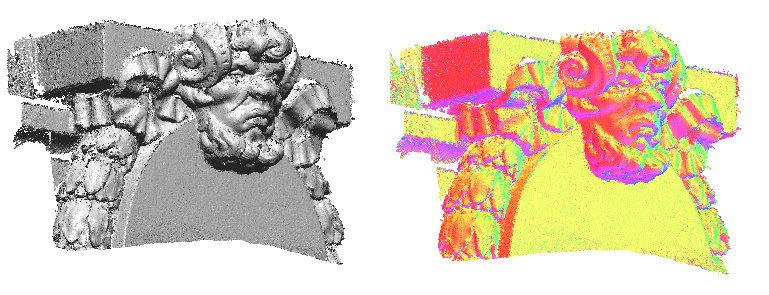
\includegraphics[width=0.65\textwidth]{Partie3_Fonctions/convertToHSV.png}
\caption{\label{fig:computeNormalsDlg}Exemple de conversion de normales vers l'espace de couleur HSV}
\end{center}
\end{figure}

La m�thode cr�� le champ \textit{Couleur} si besoin (et sinon �crase la champ existant). Elle cache aussi automatiquement les normales.